\documentclass[aspectratio=169]{beamer}

\usepackage[english]{babel}
\usepackage{microtype}
\usepackage{graphicx}
\usepackage[utf8]{inputenc}
\usepackage{amssymb,amsmath}
\usepackage{resizegather}
\usepackage{ulem}
\usepackage{epsfig}
\usepackage{color}
\usepackage{contour }
\usepackage{colortbl}
\usepackage{mystyl}
\usepackage[style=phys,articletitle=false,maxnames=4,minnames=3]{biblatex}
\bibliography{databank}
\usepackage[font=small]{caption}
\usepackage{chemfig}
\usepackage{multimedia}
% \usepackage{animation}
\usepackage{units}
\usepackage{upgreek}
\usepackage{algorithmicx}
\usepackage{algpseudocode}
\usepackage{epigraph}
\usepackage{tipa}
\usepackage{amsthm}
\usepackage{amscd}
\usepackage{wasysym}
\usepackage{subcaption}
\usepackage{soul}
\usepackage{tikz}
\def\checkmark{\tikz\fill[scale=0.4](0,.35) -- (.25,0) -- (1,.7) -- (.25,.15) -- cycle;}

\usepackage{setspace}
\newcommand{\leftcumulant}{{\langle\langle}}
\newcommand{\rightcumulant}{{\rangle\rangle}}

% Variable width example block
\newenvironment<>{varexampleblock}[2][0.9\textwidth]{%
  \setlength{\textwidth}{#1}%
  \setlength{\linewidth}{\textwidth}%
  \begin{actionenv}#3%
    \def\insertblocktitle{#2}%
    \par%
    \setbeamercolor{local structure}{parent=example text}%
    \usebeamertemplate{block example begin}}
  {\par%
    \usebeamertemplate{block example end}%
  \end{actionenv}
}

\graphicspath{{../figures/}}
\usetheme{Luebeck}
\usecolortheme{own}

\captionsetup[subfigure]{labelformat=empty}

\titlegraphic{
  \vspace{-2\baselineskip}
  \begin{columns}
    \begin{column}{0.16\textwidth}
      \begin{figure}
        \centering
        
\includegraphics[width=0.75\textwidth]{schmidt_logo}
      \end{figure}

    \end{column}
    \begin{column}{0.65\textwidth}
      \centering
      \vspace{0.5\baselineskip}
      \centering
      \begin{figure}
        \centering
        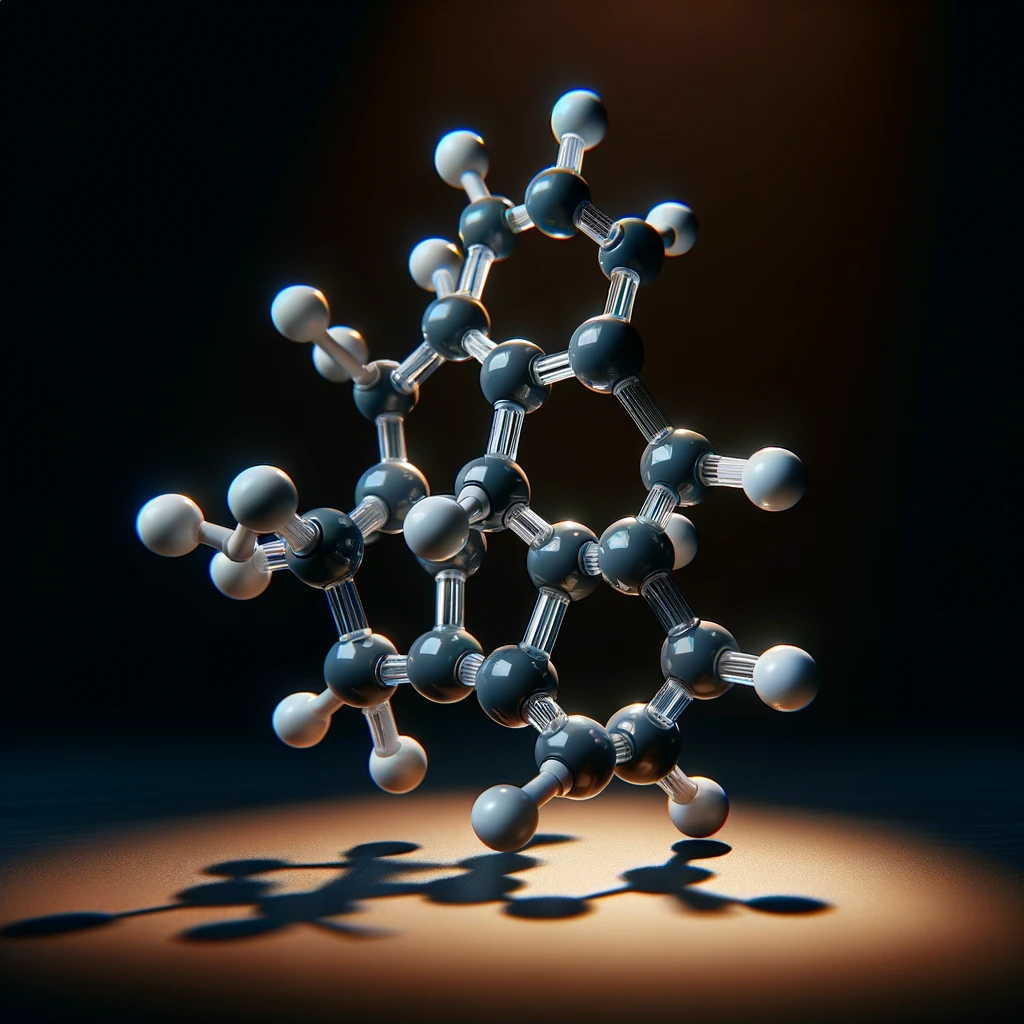
\includegraphics[width=0.25\textwidth]{image}
      \end{figure}
    \end{column}
    \begin{column}{0.16\textwidth}
      \begin{figure}
        \centering
        
\includegraphics[width=0.75\textwidth]{dsi}
      \end{figure}
    \end{column}
  \end{columns}
  \vfill
}

\title{Predicting Atom Interactions with AI}
\author[{
\includegraphics[height=0.95em]{favicon} Ludwig Schneider (he/him)}]{Ludwig Schneider}
\institute{Eric and Wendy Schmidt AI-Postdoctoral Fellowship\\Pritzker School of Molecular Engineering\\Data Science Institute University of Chicago}


\begin{document}

\frame{\titlepage\thispagestyle{empty}}
\addtocounter{framenumber}{-1}

\renewcommand\citationtext{\fullcite{jorgensen1996development}}
\section*{Introduction}
\begin{frame}
  \frametitle{Moelcular Interaction: Non-Bonded I}
  \begin{columns}
    \begin{column}{0.5\textwidth}
      \begin{itemize}
      \item Newtons Equation of Motion
      \end{itemize}
        \begin{align}
          m_i \frac{\text{d}^2}{\text{d}t^2}\vec{r_i} = \vec{F_i}\nonumber
        \end{align}
        \vspace{-0.5\baselineskip}
        \begin{itemize}
      \item determine forces $\vec{F}$
      \item OPLS: functional form for the forcefield
      \end{itemize}
      \begin{align}
        V_\text{nb}(r_{ij}) &= \epsilon_{ij} \left(\frac{\sigma_{ij}}{r_{ij}^{12}} - \frac{\sigma_{ij}}{r_{ij}^6}\right) + \frac{q_iq_j e^2}{4\pi\epsilon_0 r_{ij}}\nonumber\\
        \epsilon_{ij} &= \sqrt{\epsilon_i \epsilon_j} \quad \sigma_{ij} = \sqrt{\sigma_i \sigma_j}\nonumber
      \end{align}
      \vspace{-0.5\baselineskip}
      \alert{Challenge}: determine $\epsilon_i$, $\sigma_i$, $q_i$, and $m_i$
    \end{column}
    \begin{column}{0.5\textwidth}
      \begin{figure}
        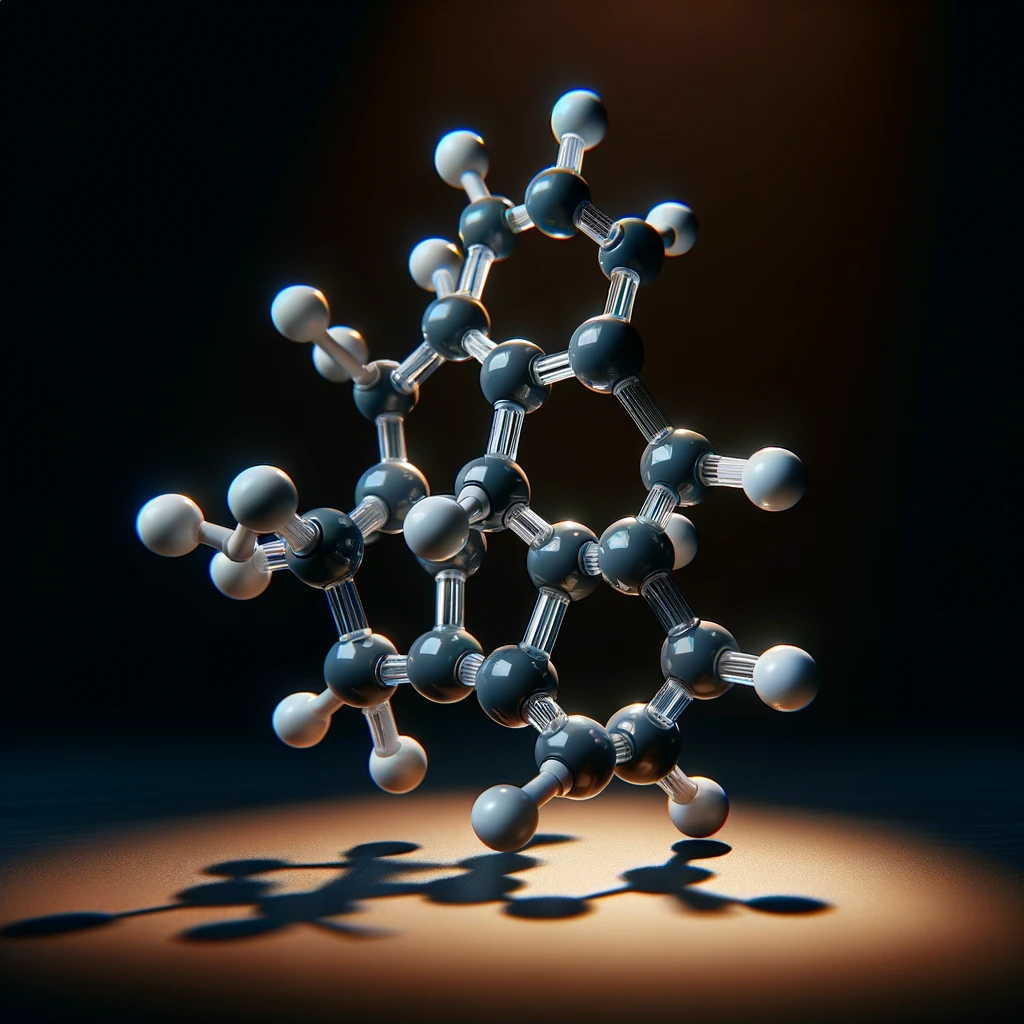
\includegraphics[width=0.75\textwidth]{image}
      \end{figure}
    \end{column}
  \end{columns}
\end{frame}

\begin{frame}
  \frametitle{Moelcular Interaction: Non-Bonded Interactions II}
  \begin{columns}
    \begin{column}{0.5\textwidth}
      \begin{itemize}
      \item determine $\epsilon_i$, $\sigma_i$, $q_i$, and $m_i$
                \begin{itemize}
        \item element (carbon, hydrogen)
        \item molecular environment
        \end{itemize}
      \item we know some values
      \item SMARTS based rules
      \item Quantum Mechanic simulations
      \item chemical space is vast, we want to interpolate
      \end{itemize}
      \begin{exampleblock}{Your Challenge}
        Use ML to interpolate from known molecules!
      \end{exampleblock}
    \end{column}
    \begin{column}{0.5\textwidth}
      \begin{figure}
        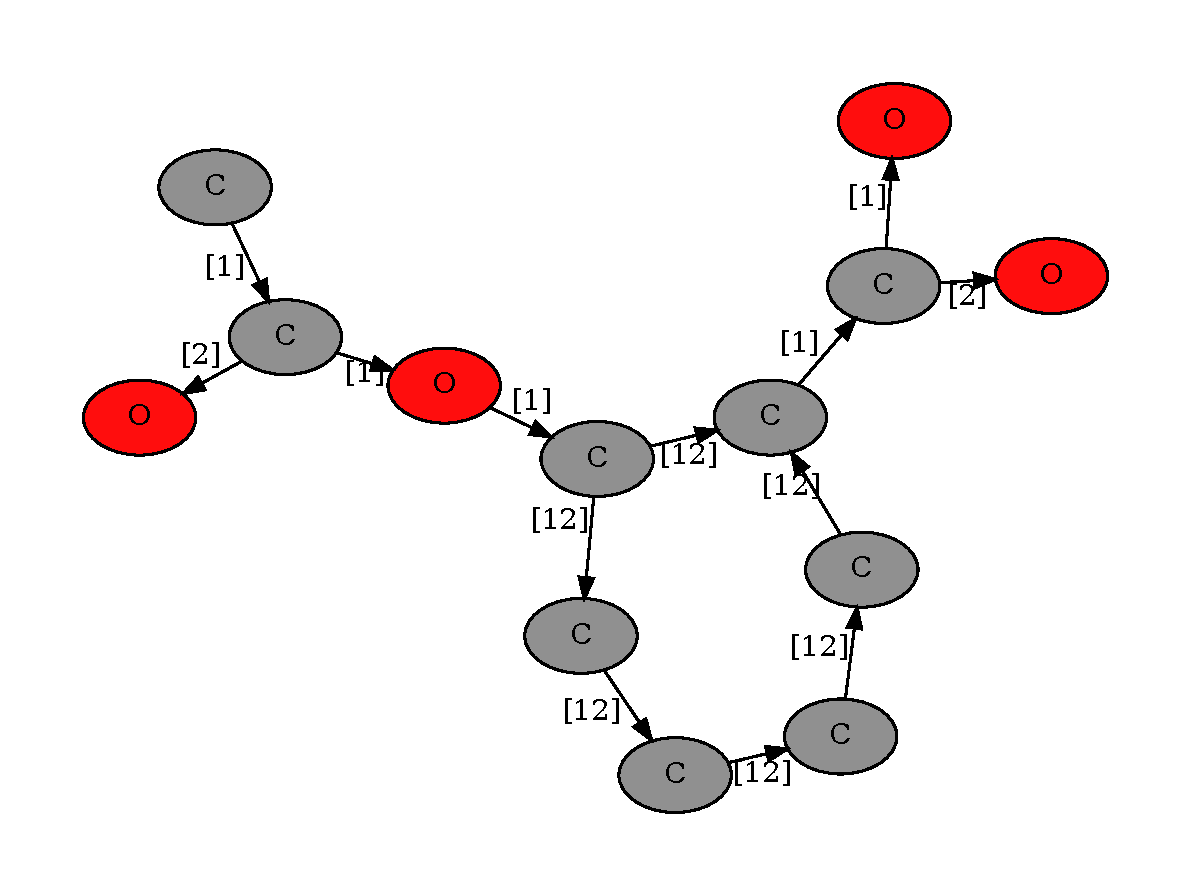
\includegraphics[width=\textwidth]{atom_graph}
      \end{figure}
    \end{column}
  \end{columns}
\end{frame}

\section{Dataset}
\renewcommand\citationtext{\url{https://github.com/uchicago-dsi/ai-sci-hackathon-2024}}
\begin{frame}
  \frametitle{Details of the Basic Challenge}
  \begin{columns}
    \begin{column}{0.48\textwidth}
      \begin{itemize}
      \item 3000 molecular graphs
      \item known input parameters
      \item supervised learning possible
        \begin{enumerate}
        \item predict non-bonded parameters
        \item predict uncertaintiy in interpolation
        \end{enumerate}
      \item you are free to choose your model
      \item you are free to choose tech stack
      \item make results permutation invariant
      \item do not rely on SMILES!
      \end{itemize}
    \end{column}
    \begin{column}{0.52\textwidth}
      \begin{itemize}
      \item \url{https://github.com/uchicago-dsi/ai-sci-hackathon-2024}
      \item \texttt{molecular/intro/talk.pdf} this slide deck
      \item \texttt{molecular/README.md} starting point
      \item \texttt{molecular/explain\_graph\_data.py} explanation of data set
      \item \texttt{molecular/data.json} training data
      \item molecular graph as \texttt{networkx} graphs
      \end{itemize}
    \end{column}
  \end{columns}
\end{frame}

\renewcommand\citationtext{\url{https://dmol.pub/dl/gnn.html}}

\begin{frame}
  \frametitle{How to get Started?}
  \begin{columns}
    \begin{column}{0.5\textwidth}
      \begin{exampleblock}{1. Understand the Data}
        \begin{itemize}
        \item visualize graphs
        \item transform to tech stack
        \end{itemize}
      \end{exampleblock}
      \begin{exampleblock}{Tech Stack Options}
        \begin{itemize}
        \item Flax/JAX with Jraph
        \item PyTorch with Torch-Geometric
        \item Tensorflow with GNN
        \end{itemize}
      \end{exampleblock}
      \begin{exampleblock}{Tools}
        \begin{itemize}
        \item visualization: \href{GraphViz - Dot}{https://graphviz.org/}
        \item python: \href{NetorkX}{https://networkx.org/}
        \end{itemize}
      \end{exampleblock}
    \end{column}
    \begin{column}{0.5\textwidth}
      \begin{itemize}
      \item New to GNN?
      \item New to Molecular AI?
      \item Dmol introduction!
      \end{itemize}
      \centering
      {\small\url{https://dmol.pub/dl/gnn.html}}
      \begin{figure}
        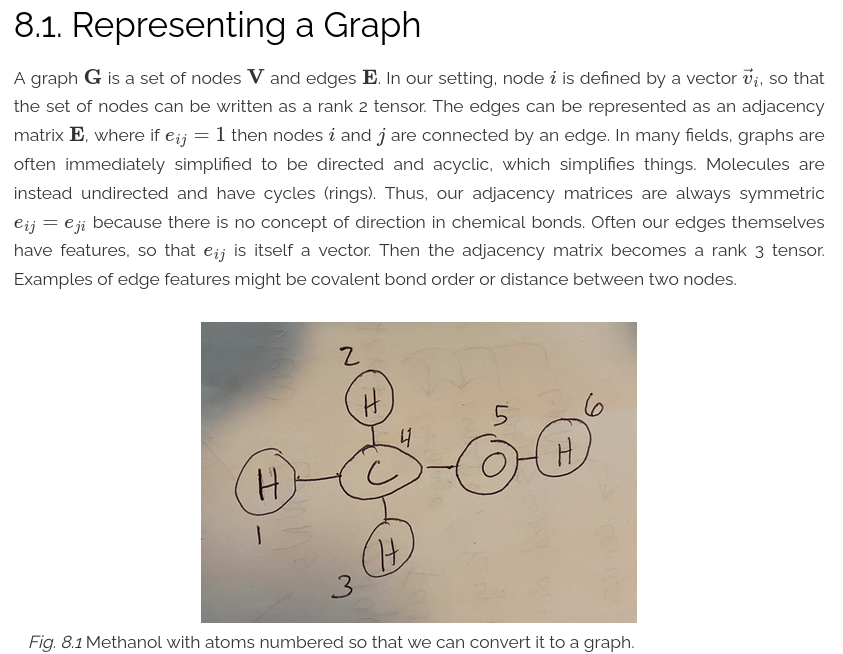
\includegraphics[width=0.75\textwidth]{dmol}
      \end{figure}
    \end{column}
  \end{columns}
\end{frame}

\renewcommand\citationtext{}
\begin{frame}
  \frametitle{How we Evaluate You!}
  \begin{columns}
    \begin{column}{0.4\textwidth}
      \begin{itemize}
      \item prepare a final presentation
      \item convince us your solution is best
      \item include model details and results
      \item 7 minutes to present
      \item 2 minutes for our questions
      \end{itemize}
    \end{column}
    \begin{column}{0.55\textwidth}
      \begin{exampleblock}{Wednesday \@ 3PM: we give you additional data}
      \end{exampleblock}
      \begin{itemize}
      \item DO NOT TRAIN with this data
      \item Send your result back as soon as you can!
      \item \texttt{molecular/final\_evaluation.py}
      \item report output in your presentation!
      \item return data by 5 PM!
      \end{itemize}
      \begin{exampleblock}{Example Test Data}
        \begin{itemize}
        \item {\footnotesize\texttt{molecular/validation\_example.json}}
        \item {\footnotesize\texttt{molecular/permutation\_example.json}}
        \item {\footnotesize\texttt{molecular/permutation\_example\_masked.json}}
        \end{itemize}
      \end{exampleblock}
    \end{column}
  \end{columns}
\end{frame}

\section{Extra Challenges}

\begin{frame}
  \frametitle{What if you solve the challenge too fast?}
  \begin{columns}
    \begin{column}{0.4\textwidth}
      \begin{exampleblock}{Traditional}
        \begin{itemize}
        \item predict bond class for atom
        \item look-up table for parameters
        \item \texttt{ffbonded.itp}
        \end{itemize}
      \end{exampleblock}
        \begin{exampleblock}{GNN approach}
          \begin{itemize}
          \item predict parameters directly
          \item bonds: edge features
          \item angles \& dihedrals \alert{?}
          \end{itemize}
        \end{exampleblock}
    \end{column}
    \begin{column}{0.55\textwidth}
      \begin{itemize}
      \item bonds: 2 atoms: 2 parameters
      \end{itemize}
      \begin{align}
        V_b(r_{ij}) = k_{a} (r_{ij} - b_{0})^2 \nonumber
      \end{align}
      \begin{itemize}
      \item angles: 3 atoms: 2 parameters
      \end{itemize}
      \begin{align}
        V_a(\theta) = k_{\theta} (\theta - \theta_0)^2 \quad \theta = \cos^{-1}( \vec{r_{ij}} \cdot \vec{r_{jk}} /(||\vec{r_{ij}}|| ||\vec{r_{jk}}||))\nonumber
      \end{align}
      \begin{itemize}
      \item dihedral: 4 atoms: 8 parameters
      \end{itemize}
      \begin{align}
        V_d(\phi) = \sum_{i=1,2,3,4} V_i/2[1- (-1)^i\cos(i \cdot \phi-\phi_i)]\nonumber
      \end{align}
    \end{column}
  \end{columns}
\end{frame}

\section*{Thank you for your attention!}
\renewcommand\Switch{0}
\renewcommand\citationtext{}
\subsection*{Questions?}

\begin{frame}
  \frametitle{Happy Hacking!}

  \centering
  \Huge{Questions?}
\end{frame}
\beginbackup


\label{fr:appendix}
\appendix

% \begin{frame}[allowframebreaks,noframenumbering]
%   \frametitle{References}
%   \printbibliography
% \end{frame}

\section{Backup slides}

\section*{The End}
\renewcommand\citationtext{}
\backupend
\end{document}

%%% Local Variables:
%%% mode: latex
%%% TeX-master: t
%%% End:
